\documentclass[10pt,a4paper]{article}
\usepackage[utf8]{inputenc}
\usepackage{amsmath}
\usepackage{float}
\usepackage{physics}
\usepackage{graphicx}
\usepackage{hyperref}

\author{Mikael B. Kiste}
\title{FYS5100 - project 1}

\begin{document}
    \maketitle

    \abstract In this project various numerical procedures to solve linear equations has been implemented. The relative performance of these procedures in terms of efficiency, numerical stability and numerical precision has been evaluated.

    \tableofcontents

    \newpage
    \section{Introduction}
    Differential equations appear in almost all fields of physics and are essential in understanding how physical systems evolve. Since analytical and general solutions to differential equations are notoriously difficult to find it is often useful to approach these problems numerically instead. Solving sets of linear equations through gaussian elimination is a repetitive step by step process expertly handled by computers. In section 1 an implementable algorithm for solving a simple tridiagonal matrix is derived. In the following sections we look at how solutions to the general one-dimensional Poisson differential equation can be translated into linear equations that manifest as a special tridiagonal matrix. New and improved algorithms solving this specific system are derived before being compared with the general algorithms. \footnote{sourcecode can be found at https://github.com/mikaelbk/fys3150-project-1}

	\newpage
    \section{Numerical solution for a linear system comprising of a tridiagonal matrix}
    Consider the following system of linear equations
	$$\vb{Av} = \vb{u}$$
	Where $\vb{A}$ is an nxn tridiagonal matrix and $\vb{v}$ and $\vb{u}$ are vectors of length n.
    We want a solution for $\vb{v}$ expressed through the elements of $\vb{A}$ and $\vb{u}$.
    We conduct a standard gaussian elimination process initially by forward substitution, which eliminates the leading entry on all but the first row, and thereby using backward substitution which leaves a single entry on each row and a solution is reached. For clarity let the three different diagonals consist of indexed elements of a, b and c

    \[
    \begin{bmatrix}
    b_1 & c_1 &  &  &  \\
    a_1 & b_2 & c_2 &  &  \\
    & a_2 & \ddots & \ddots &  \\
    &  & \ddots & \ddots & c_{n-1} \\
    &  &  & a_{n-1} & b_n
    \end{bmatrix}
    \begin{bmatrix}
	    v_1 \\
	    v_2 \\
	    \vdots \\
	    v_{n-1} \\
	    v_n
    \end{bmatrix} =
    \begin{bmatrix}
	    u_1 \\
	    u_2 \\
	    \vdots \\
	    u_{n-1} \\
	    u_n
    \end{bmatrix}
    \]
    The first operation is to subtract row one times $a_1/b_1$ from the second row. This eliminates $a_1$ on the second row. This, however, leads to two new elements where $b_2$ and $u_2$ currently lie.
    \[
    \begin{bmatrix}
        b_1 & c_1 & 0 & \dots\\
        0 & b_2-\tfrac{a_1}{b_1}c_1 & c_2 & \dots\\
        \vdots & \vdots & \vdots & \ddots
    \end{bmatrix}
    \begin{bmatrix}
        v_1\\
        v_2\\
        \vdots
    \end{bmatrix}
    =
    \begin{bmatrix}
        u_1\\
        u_2-\tfrac{a_1}{b_1}u_1\\
        \vdots
    \end{bmatrix}
    \]
    If the new elements are renamed to $\tilde{b}_2 = b_2-\tfrac{a_1}{b_1} $ and $\tilde{u}_2 = u_2-\tfrac{a_1}{b_1}u_1$ we can continue with the forwards substitution until the n'th element and get a general expression for the new $\tilde{b}_i$'s and $\tilde{u}_i$'s
    \[
    \begin{bmatrix}
    \tilde{b}_1 & c_1 &  &  &  \\
    0 & \tilde{b}_2 & c_2 &  &  \\
    & 0 & \ddots & \ddots &  \\
    &  & \ddots & \ddots & c_{n-1} \\
    &  &  & 0 & \tilde{b}_n
    \end{bmatrix}
    \begin{bmatrix}
        v_1 \\
        v_2 \\
        \vdots \\
        v_{n-1} \\
        v_n
    \end{bmatrix} =
    \begin{bmatrix}
        u_1 \\
        \tilde{u}_2 \\
        \vdots \\
        \tilde{u}_{n-1} \\
        \tilde{u}_n
    \end{bmatrix}
    \]
    where
    \begin{align}
    \tilde{b}_i = b_i - \tfrac{a_{i-1}}{\tilde{b}_{i-1}}c_{i-1}\\
    \tilde{u}_i = u_i - \tfrac{a_{i-1}}{\tilde{b}_{i-1}}\tilde{u}_{i-1}
    \end{align}

    At this point we see that we actually have a solution for the last element. $\tilde{b}_n v_n = \tilde{u}_n$ And by backwards substitution we can solve for all the other $v_i$'s.
    \begin{equation}
    v_i = \frac{\tilde{u}_i-c_iv_{i+1}}{\tilde{b}_i}, \quad v_n = \tilde{u}_n/\tilde{b}_n
    \end{equation}

	\newpage
    \section{Differential equations as a linear problem}
    The general one-dimensional Poisson equation can be expressed as
    \[
    -g''(x) = f(x)
    \]
    We want to find $g''(x)$ with boundary conditions $g(0) = g(1)$ and in the variable domain $x\in (0\leq x<1)$ for some $f(x)$
    We can do this by discretization. Let $u_i$ and $v_i$ be the elements of a discretized $f(x)$ and $g(x)$, respectively. We can write the second derivative as
    $$-\frac{v_{i+1}+v_{i-1}-2v_i}{h^2} = u_i, \qquad i = 1,2,...,n$$
    This is a series of equations for all the values of i. By rearanging some of the terms and multiplying with $h^2$ they can be written as such
    \begin{align*}
        -v_0 + 2v_1 - v_2 &= h^2u_1\\
        -v_1 + 2v_2 - v_3 &= h^2u_2\\
        -v_2 + 2v_3 - v_4 &= h^2u_3\\
        &\vdots\\
        -v_{n-2} + 2v_{n-1} - v_{n} &= h^2u_{n-1}\\
        -v_{n-1} + 2v_{n} - v_{n+1} &= h^2u_{n}\\
    \end{align*}
    But from the boundary conditions we know that $v_0 = v_{n+1} = 0$, so we can exclude them and solve for the rest of the system. Expressed on matrix form we get

    \begin{equation}\label{special matrix}
    \begin{bmatrix}
    2 & -1 & 0 & \dots & 0 & 0 & 0 \\
    -1 & 2 & -1 & \dots & 0 & 0 & 0 \\
    \vdots & \vdots & \vdots & \ddots & 0 & 0 & 0 \\
    0 & 0 & 0 & 0 & -1 & 2 & -1\\
    0 & 0 & 0 & 0 & 0 & -1 & 2 \\
    \end{bmatrix}
    \begin{bmatrix}
        v_1\\ v_2 \\ v_3 \\ \vdots \\ v_{n-2} \\v_{n-1} \\ v_{n}
    \end{bmatrix}
    =h^2
    \begin{bmatrix}
        u_1 \\ u_2 \\ u_3 \\ \vdots \\ u_{n-2} \\ u_{n-1} \\ u_{n}
    \end{bmatrix}
    \end{equation}

    This is the same problem that was solved for in the previous section with the notable exception that the diagonals have some special values. It is therefore beneficial to write a simplified algorithm that abuses these values as this leads to fewer FLOPS.
https://github.com/mikaelbk/fys3150-project-1
	\newpage
    \section{Specific numerical solution}
    We begin with gaussian elimination on the matrix in equation (\ref{special matrix}) mentioned in the previous section. First we want to add half of the first row to the second row, as this eliminates the leading -1 on the second row. Next we want to eliminate the -1 on row three, but since row two changed we now need to add two thirds of row two to row three instead. If one continues with this process, a pattern emerges
    \begin{align*}
    \begin{bmatrix}
    2 & -1 & 0 & 0 & \dots & 0 & 0 & 0 \\
    0 & 2-\tfrac{1}{2} & -1 & 0 & \dots & 0 & 0 & 0 \\
    0 & 0 & 2-\tfrac{2}{3} & -1 & \dots & 0 & 0 & 0 \\
    \vdots & \vdots & \vdots & \vdots & \ddots & 0 & 0 & 0 \\
    0 & 0 & 0 & 0 & 0 & 0 & 2 - \tfrac{n-2}{n-1} & -1\\
    0 & 0 & 0 & 0 & 0 & 0 & 0 & 2 - \tfrac{n-1}{n} \\
    \end{bmatrix}
    \begin{bmatrix}
        v_1\\ v_2 \\ v_3 \\ v_4 \\ \vdots \\ v_{n-2} \\v_{n-1} \\ v_{n}
    \end{bmatrix}
    =h^2
    \begin{bmatrix}
        u_1 \\ u_2 + u_1\tfrac{1}{2} \\ \tilde{u}_3 \\ \tilde{u}_4 \\ \vdots \\ \tilde{u}_{n-2} \\ \tilde{u}_{n-1} \\ \tilde{u}_{n}
    \end{bmatrix}
    \end{align*}
    Now we have a general expression for the diagonal elements that does not depend on previous values, i.e. $\tilde{b}_i$ is not a function of $\tilde{b}_{i-1}$. Instead we have
    \begin{align}
        \tilde{b}_i = 2 - \frac{i-1}{i} = \frac{2i-(i-1)}{i} =\frac{i+1}{i}\\
        \tilde{u}_i = u_i + \tilde{u}_{i-1}\tfrac{i-1}{i}
    \end{align}
    Now for the backwards substitution we have
    \begin{align}
    v_n = \tilde{u}_n\frac{n}{n+1}\\
    v_{i}\frac{i+1}{i} - v_{i+1} = \tilde{u}_{i} \implies v_i =(\tilde{u}_i+v_{i+1})\frac{i}{i+1}
    \end{align}

    \newpage{}
    \section{FLOP evaluation}
    Now that we have expressions for how to calculate the different values of $v_i$ it is time to actually implement this and evaluate how the different algorithms compare to one another.
    For the general it is easy to see that we have 6 floating point operations (basic arithmetic operations with float datatype numbers) in equation 1 and 2, 3 in each. And 2 FLOPS for equation 3. All in all 8 FLOPS.
    However, since we do not need to apply this for the very first element (e.g. $\tilde{b}_1 = b_1$) we can subtract one loop iteration. If we have an $n\times n$ matrix the number of FLOPS then becomes $8(n-1)$.\\
    For the special algorithm we can abuse the fact that have an analytical term that saves us one operation in the forwards substitution and one in the backwards substitution. Therefore we have $6(n-1)$ FLOPS in the specific numerical solution.

    \newpage{}
    \section{Results}
    Results are presented through plots in this section.
    \begin{figure}
      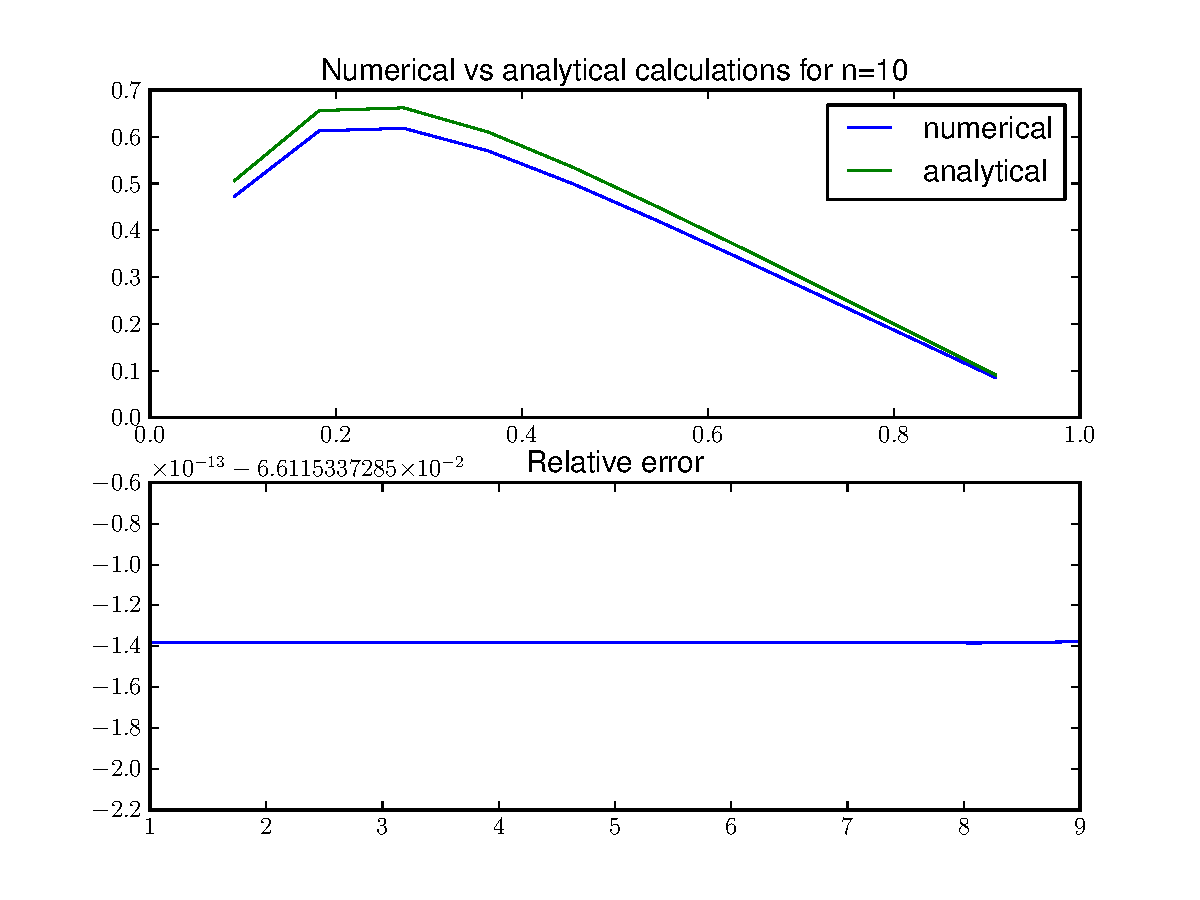
\includegraphics[width = \textwidth]{general_10}
      \caption{This is the plot for n=10 using the general algorithm. There is quite some difference between the numerical vs the analytical solution}
    \end{figure}
    \begin{figure}
      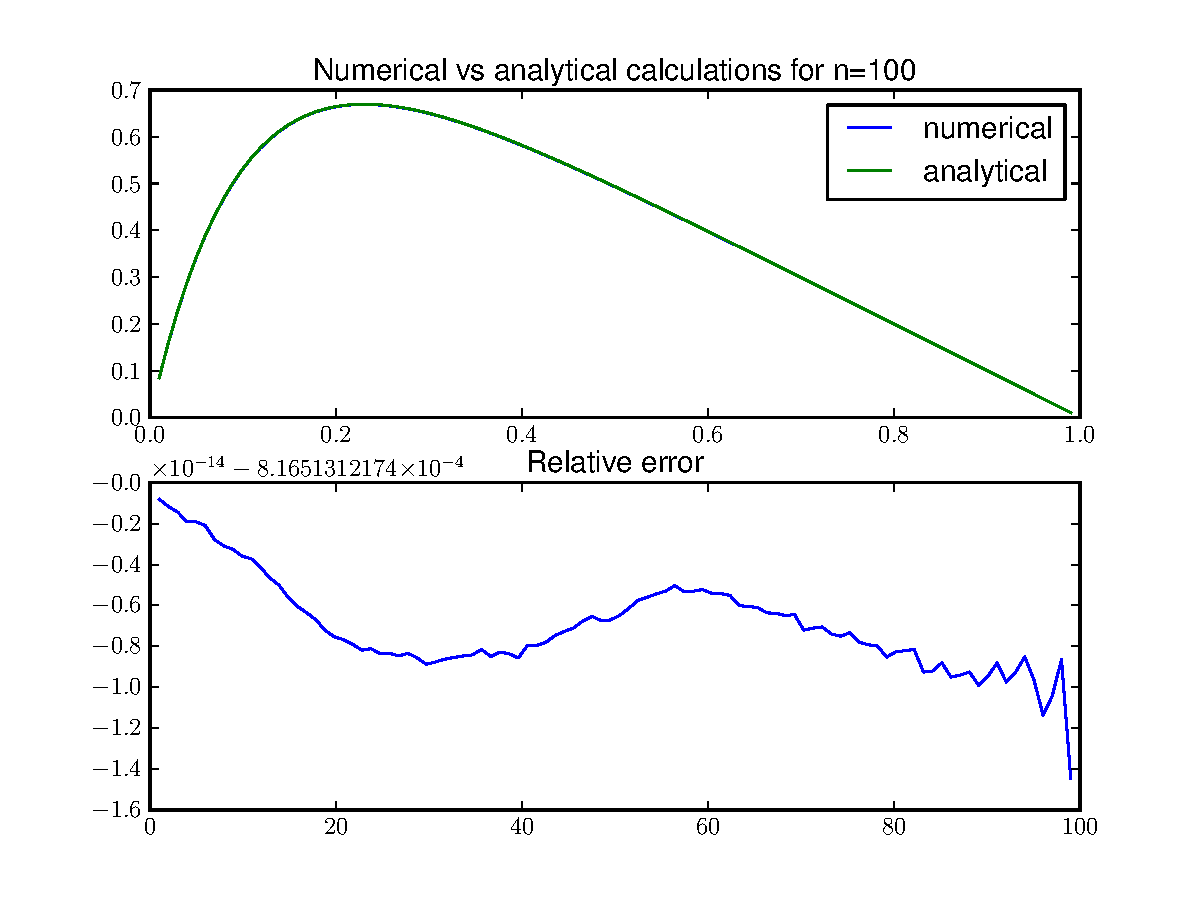
\includegraphics[width = \textwidth]{general_100}
      \caption{This is the plot for n=100 using the general algorithm. The difference between the numerical vs the analytical solution only shows in a log plot of the relative error}
    \end{figure}
    \begin{figure}
      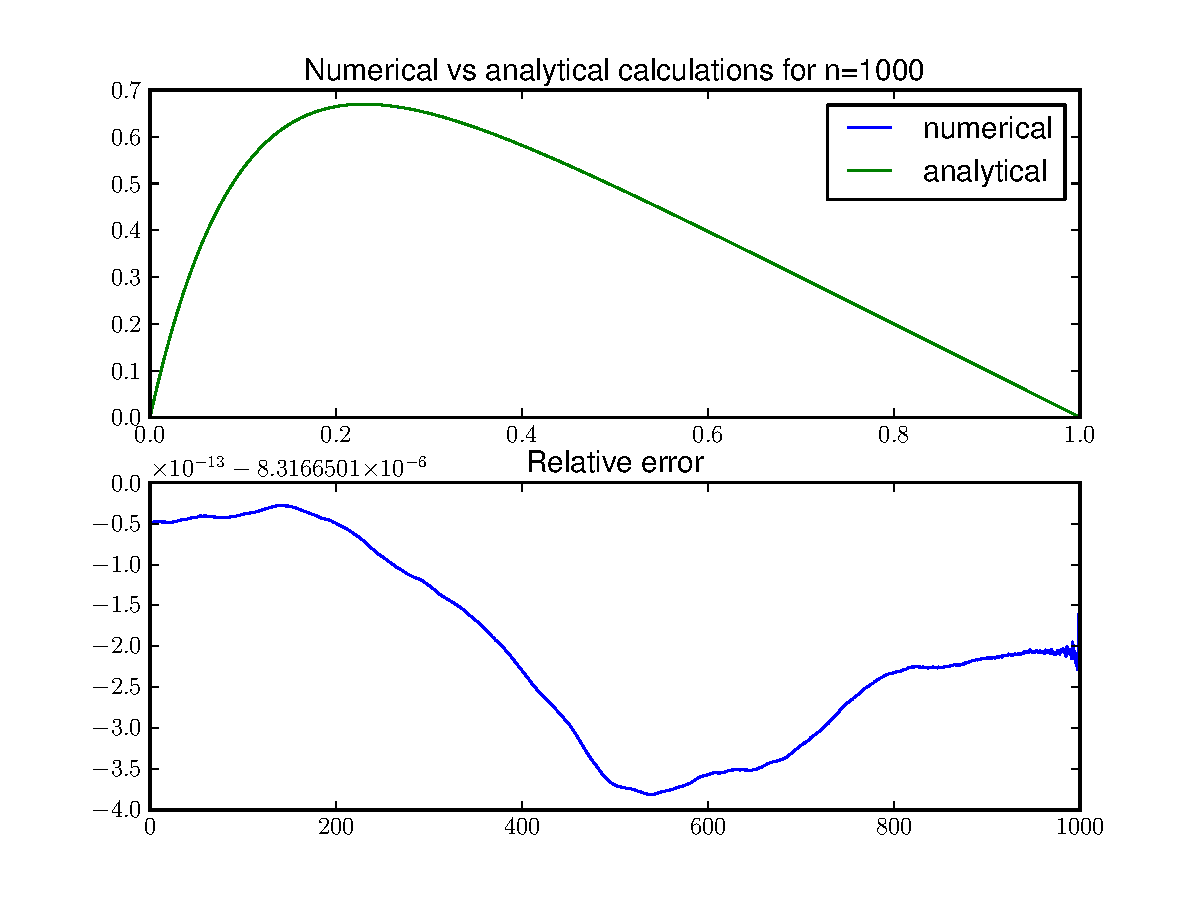
\includegraphics[width = \textwidth]{general_1000}
      \caption{This is the plot for n=1000 using the general algorithm. The difference between the numerical vs the analytical solution is miniscule}
    \end{figure}

    \newpage{}
    \section{Discussion}
    From figure 1, 2 and 3 there is a trend that the numerical solution gets more and more accurate for more datapoints. For only 10 there is almost too much variance to consider the results as even indicative.

    \newpage{}
    \section{sources}
    \begin{itemize}
     \item
     \href{https://github.com/CompPhysics/ComputationalPhysics}{fys3150 github repo}
     \item \href{http://www.uio.no/studier/emner/matnat/fys/FYS3150/h17/index.html}{fys3150 course page}
    \end{itemize}

\end{document}
